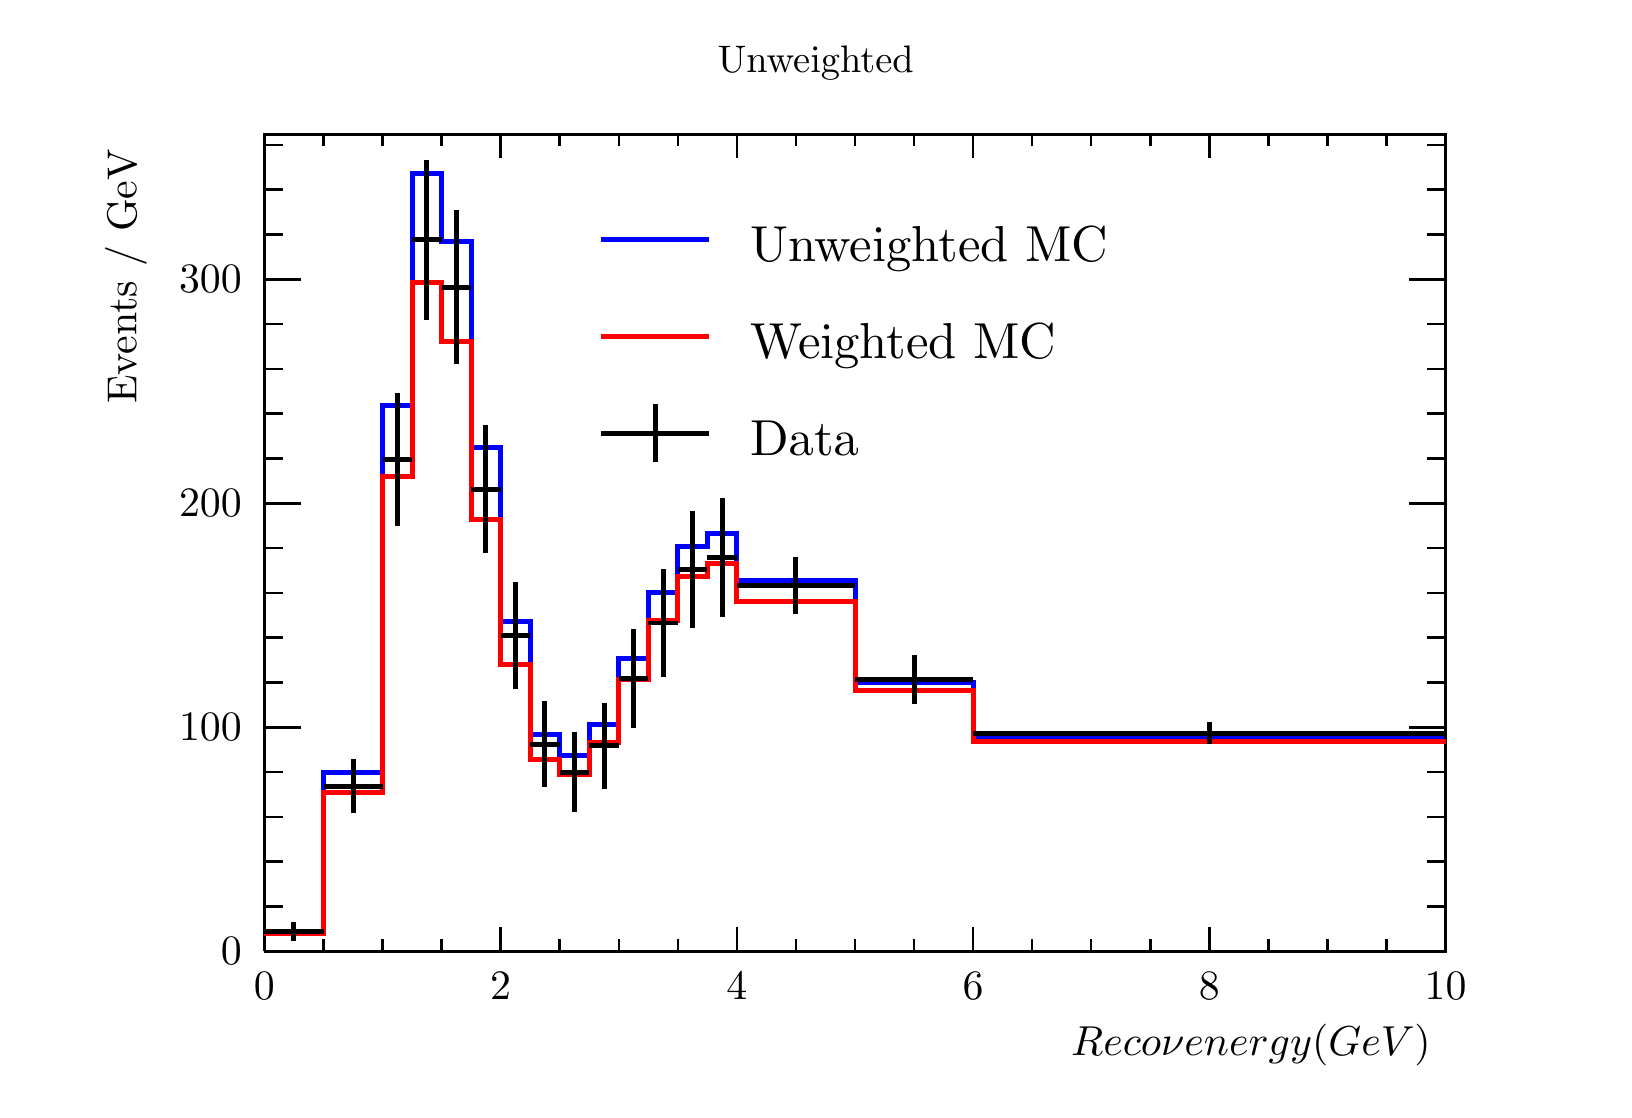
\begin{tikzpicture}
\pgfdeclareplotmark{cross} {
\pgfpathmoveto{\pgfpoint{-0.3\pgfplotmarksize}{\pgfplotmarksize}}
\pgfpathlineto{\pgfpoint{+0.3\pgfplotmarksize}{\pgfplotmarksize}}
\pgfpathlineto{\pgfpoint{+0.3\pgfplotmarksize}{0.3\pgfplotmarksize}}
\pgfpathlineto{\pgfpoint{+1\pgfplotmarksize}{0.3\pgfplotmarksize}}
\pgfpathlineto{\pgfpoint{+1\pgfplotmarksize}{-0.3\pgfplotmarksize}}
\pgfpathlineto{\pgfpoint{+0.3\pgfplotmarksize}{-0.3\pgfplotmarksize}}
\pgfpathlineto{\pgfpoint{+0.3\pgfplotmarksize}{-1.\pgfplotmarksize}}
\pgfpathlineto{\pgfpoint{-0.3\pgfplotmarksize}{-1.\pgfplotmarksize}}
\pgfpathlineto{\pgfpoint{-0.3\pgfplotmarksize}{-0.3\pgfplotmarksize}}
\pgfpathlineto{\pgfpoint{-1.\pgfplotmarksize}{-0.3\pgfplotmarksize}}
\pgfpathlineto{\pgfpoint{-1.\pgfplotmarksize}{0.3\pgfplotmarksize}}
\pgfpathlineto{\pgfpoint{-0.3\pgfplotmarksize}{0.3\pgfplotmarksize}}
\pgfpathclose
\pgfusepathqstroke
}
\pgfdeclareplotmark{cross*} {
\pgfpathmoveto{\pgfpoint{-0.3\pgfplotmarksize}{\pgfplotmarksize}}
\pgfpathlineto{\pgfpoint{+0.3\pgfplotmarksize}{\pgfplotmarksize}}
\pgfpathlineto{\pgfpoint{+0.3\pgfplotmarksize}{0.3\pgfplotmarksize}}
\pgfpathlineto{\pgfpoint{+1\pgfplotmarksize}{0.3\pgfplotmarksize}}
\pgfpathlineto{\pgfpoint{+1\pgfplotmarksize}{-0.3\pgfplotmarksize}}
\pgfpathlineto{\pgfpoint{+0.3\pgfplotmarksize}{-0.3\pgfplotmarksize}}
\pgfpathlineto{\pgfpoint{+0.3\pgfplotmarksize}{-1.\pgfplotmarksize}}
\pgfpathlineto{\pgfpoint{-0.3\pgfplotmarksize}{-1.\pgfplotmarksize}}
\pgfpathlineto{\pgfpoint{-0.3\pgfplotmarksize}{-0.3\pgfplotmarksize}}
\pgfpathlineto{\pgfpoint{-1.\pgfplotmarksize}{-0.3\pgfplotmarksize}}
\pgfpathlineto{\pgfpoint{-1.\pgfplotmarksize}{0.3\pgfplotmarksize}}
\pgfpathlineto{\pgfpoint{-0.3\pgfplotmarksize}{0.3\pgfplotmarksize}}
\pgfpathclose
\pgfusepathqfillstroke
}
\pgfdeclareplotmark{newstar} {
\pgfpathmoveto{\pgfqpoint{0pt}{\pgfplotmarksize}}
\pgfpathlineto{\pgfqpointpolar{44}{0.5\pgfplotmarksize}}
\pgfpathlineto{\pgfqpointpolar{18}{\pgfplotmarksize}}
\pgfpathlineto{\pgfqpointpolar{-20}{0.5\pgfplotmarksize}}
\pgfpathlineto{\pgfqpointpolar{-54}{\pgfplotmarksize}}
\pgfpathlineto{\pgfqpointpolar{-90}{0.5\pgfplotmarksize}}
\pgfpathlineto{\pgfqpointpolar{234}{\pgfplotmarksize}}
\pgfpathlineto{\pgfqpointpolar{198}{0.5\pgfplotmarksize}}
\pgfpathlineto{\pgfqpointpolar{162}{\pgfplotmarksize}}
\pgfpathlineto{\pgfqpointpolar{134}{0.5\pgfplotmarksize}}
\pgfpathclose
\pgfusepathqstroke
}
\pgfdeclareplotmark{newstar*} {
\pgfpathmoveto{\pgfqpoint{0pt}{\pgfplotmarksize}}
\pgfpathlineto{\pgfqpointpolar{44}{0.5\pgfplotmarksize}}
\pgfpathlineto{\pgfqpointpolar{18}{\pgfplotmarksize}}
\pgfpathlineto{\pgfqpointpolar{-20}{0.5\pgfplotmarksize}}
\pgfpathlineto{\pgfqpointpolar{-54}{\pgfplotmarksize}}
\pgfpathlineto{\pgfqpointpolar{-90}{0.5\pgfplotmarksize}}
\pgfpathlineto{\pgfqpointpolar{234}{\pgfplotmarksize}}
\pgfpathlineto{\pgfqpointpolar{198}{0.5\pgfplotmarksize}}
\pgfpathlineto{\pgfqpointpolar{162}{\pgfplotmarksize}}
\pgfpathlineto{\pgfqpointpolar{134}{0.5\pgfplotmarksize}}
\pgfpathclose
\pgfusepathqfillstroke
}
\definecolor{c}{rgb}{1,1,1};
\draw [color=c, fill=c] (0,0) rectangle (20,13.4752);
\draw [color=c, fill=c] (3,1.75177) rectangle (18,12.1277);
\definecolor{c}{rgb}{0,0,0};
\draw [c,line width=0.9] (3,1.75177) -- (3,12.1277) -- (18,12.1277) -- (18,1.75177) -- (3,1.75177);
\definecolor{c}{rgb}{1,1,1};
\draw [color=c, fill=c] (3,1.75177) rectangle (18,12.1277);
\definecolor{c}{rgb}{0,0,0};
\draw [c,line width=0.9] (3,1.75177) -- (3,12.1277) -- (18,12.1277) -- (18,1.75177) -- (3,1.75177);
\definecolor{c}{rgb}{0,0,1};
\draw [c,line width=1.8] (3,2.00296) -- (3.75,2.00296) -- (3.75,4.02844) -- (4.5,4.02844) -- (4.5,8.67764) -- (4.875,8.67764) -- (4.875,11.6336) -- (5.25,11.6336) -- (5.25,10.7727) -- (5.625,10.7727) -- (5.625,8.14604) -- (6,8.14604) -- (6,5.93854)
 -- (6.375,5.93854) -- (6.375,4.50359) -- (6.75,4.50359) -- (6.75,4.23451) -- (7.125,4.23451) -- (7.125,4.62746) -- (7.5,4.62746) -- (7.5,5.47245) -- (7.875,5.47245) -- (7.875,6.30616) -- (8.25,6.30616) -- (8.25,6.89433) -- (8.625,6.89433) --
 (8.625,7.05205) -- (9,7.05205) -- (9,6.46607) -- (10.5,6.46607) -- (10.5,5.16752) -- (12,5.16752) -- (12,4.47954) -- (18,4.47954);
\definecolor{c}{rgb}{0,0,0};
\draw [c,line width=0.9] (3,1.75177) -- (18,1.75177);
\draw [c,line width=0.9] (3,2.05496) -- (3,1.75177);
\draw [c,line width=0.9] (3.75,1.90337) -- (3.75,1.75177);
\draw [c,line width=0.9] (4.5,1.90337) -- (4.5,1.75177);
\draw [c,line width=0.9] (5.25,1.90337) -- (5.25,1.75177);
\draw [c,line width=0.9] (6,2.05496) -- (6,1.75177);
\draw [c,line width=0.9] (6.75,1.90337) -- (6.75,1.75177);
\draw [c,line width=0.9] (7.5,1.90337) -- (7.5,1.75177);
\draw [c,line width=0.9] (8.25,1.90337) -- (8.25,1.75177);
\draw [c,line width=0.9] (9,2.05496) -- (9,1.75177);
\draw [c,line width=0.9] (9.75,1.90337) -- (9.75,1.75177);
\draw [c,line width=0.9] (10.5,1.90337) -- (10.5,1.75177);
\draw [c,line width=0.9] (11.25,1.90337) -- (11.25,1.75177);
\draw [c,line width=0.9] (12,2.05496) -- (12,1.75177);
\draw [c,line width=0.9] (12.75,1.90337) -- (12.75,1.75177);
\draw [c,line width=0.9] (13.5,1.90337) -- (13.5,1.75177);
\draw [c,line width=0.9] (14.25,1.90337) -- (14.25,1.75177);
\draw [c,line width=0.9] (15,2.05496) -- (15,1.75177);
\draw [c,line width=0.9] (15.75,1.90337) -- (15.75,1.75177);
\draw [c,line width=0.9] (16.5,1.90337) -- (16.5,1.75177);
\draw [c,line width=0.9] (17.25,1.90337) -- (17.25,1.75177);
\draw [c,line width=0.9] (18,2.05496) -- (18,1.75177);
\draw [anchor=base] (3,1.14539) node[scale=1.51215, color=c, rotate=0]{0};
\draw [anchor=base] (6,1.14539) node[scale=1.51215, color=c, rotate=0]{2};
\draw [anchor=base] (9,1.14539) node[scale=1.51215, color=c, rotate=0]{4};
\draw [anchor=base] (12,1.14539) node[scale=1.51215, color=c, rotate=0]{6};
\draw [anchor=base] (15,1.14539) node[scale=1.51215, color=c, rotate=0]{8};
\draw [anchor=base] (18,1.14539) node[scale=1.51215, color=c, rotate=0]{10};
\draw [anchor= east] (18,0.565957) node[scale=1.51215, color=c, rotate=0]{$Reco \nu energy (GeV)$};
\draw [c,line width=0.9] (3,12.1277) -- (18,12.1277);
\draw [c,line width=0.9] (3,11.8245) -- (3,12.1277);
\draw [c,line width=0.9] (3.75,11.9761) -- (3.75,12.1277);
\draw [c,line width=0.9] (4.5,11.9761) -- (4.5,12.1277);
\draw [c,line width=0.9] (5.25,11.9761) -- (5.25,12.1277);
\draw [c,line width=0.9] (6,11.8245) -- (6,12.1277);
\draw [c,line width=0.9] (6.75,11.9761) -- (6.75,12.1277);
\draw [c,line width=0.9] (7.5,11.9761) -- (7.5,12.1277);
\draw [c,line width=0.9] (8.25,11.9761) -- (8.25,12.1277);
\draw [c,line width=0.9] (9,11.8245) -- (9,12.1277);
\draw [c,line width=0.9] (9.75,11.9761) -- (9.75,12.1277);
\draw [c,line width=0.9] (10.5,11.9761) -- (10.5,12.1277);
\draw [c,line width=0.9] (11.25,11.9761) -- (11.25,12.1277);
\draw [c,line width=0.9] (12,11.8245) -- (12,12.1277);
\draw [c,line width=0.9] (12.75,11.9761) -- (12.75,12.1277);
\draw [c,line width=0.9] (13.5,11.9761) -- (13.5,12.1277);
\draw [c,line width=0.9] (14.25,11.9761) -- (14.25,12.1277);
\draw [c,line width=0.9] (15,11.8245) -- (15,12.1277);
\draw [c,line width=0.9] (15.75,11.9761) -- (15.75,12.1277);
\draw [c,line width=0.9] (16.5,11.9761) -- (16.5,12.1277);
\draw [c,line width=0.9] (17.25,11.9761) -- (17.25,12.1277);
\draw [c,line width=0.9] (18,11.8245) -- (18,12.1277);
\draw [c,line width=0.9] (3,1.75177) -- (3,12.1277);
\draw [c,line width=0.9] (3.462,1.75177) -- (3,1.75177);
\draw [c,line width=0.9] (3.231,2.32073) -- (3,2.32073);
\draw [c,line width=0.9] (3.231,2.88969) -- (3,2.88969);
\draw [c,line width=0.9] (3.231,3.45865) -- (3,3.45865);
\draw [c,line width=0.9] (3.231,4.02761) -- (3,4.02761);
\draw [c,line width=0.9] (3.462,4.59656) -- (3,4.59656);
\draw [c,line width=0.9] (3.231,5.16552) -- (3,5.16552);
\draw [c,line width=0.9] (3.231,5.73448) -- (3,5.73448);
\draw [c,line width=0.9] (3.231,6.30344) -- (3,6.30344);
\draw [c,line width=0.9] (3.231,6.8724) -- (3,6.8724);
\draw [c,line width=0.9] (3.462,7.44136) -- (3,7.44136);
\draw [c,line width=0.9] (3.231,8.01031) -- (3,8.01031);
\draw [c,line width=0.9] (3.231,8.57927) -- (3,8.57927);
\draw [c,line width=0.9] (3.231,9.14823) -- (3,9.14823);
\draw [c,line width=0.9] (3.231,9.71719) -- (3,9.71719);
\draw [c,line width=0.9] (3.462,10.2861) -- (3,10.2861);
\draw [c,line width=0.9] (3.462,10.2861) -- (3,10.2861);
\draw [c,line width=0.9] (3.231,10.8551) -- (3,10.8551);
\draw [c,line width=0.9] (3.231,11.4241) -- (3,11.4241);
\draw [c,line width=0.9] (3.231,11.993) -- (3,11.993);
\draw [anchor= east] (2.9,1.75177) node[scale=1.51215, color=c, rotate=0]{0};
\draw [anchor= east] (2.9,4.59656) node[scale=1.51215, color=c, rotate=0]{100};
\draw [anchor= east] (2.9,7.44136) node[scale=1.51215, color=c, rotate=0]{200};
\draw [anchor= east] (2.9,10.2861) node[scale=1.51215, color=c, rotate=0]{300};
\draw [anchor= east] (1.24,12.1277) node[scale=1.51215, color=c, rotate=90]{Events / GeV};
\draw [c,line width=0.9] (18,1.75177) -- (18,12.1277);
\draw [c,line width=0.9] (17.538,1.75177) -- (18,1.75177);
\draw [c,line width=0.9] (17.769,2.32073) -- (18,2.32073);
\draw [c,line width=0.9] (17.769,2.88969) -- (18,2.88969);
\draw [c,line width=0.9] (17.769,3.45865) -- (18,3.45865);
\draw [c,line width=0.9] (17.769,4.02761) -- (18,4.02761);
\draw [c,line width=0.9] (17.538,4.59656) -- (18,4.59656);
\draw [c,line width=0.9] (17.769,5.16552) -- (18,5.16552);
\draw [c,line width=0.9] (17.769,5.73448) -- (18,5.73448);
\draw [c,line width=0.9] (17.769,6.30344) -- (18,6.30344);
\draw [c,line width=0.9] (17.769,6.8724) -- (18,6.8724);
\draw [c,line width=0.9] (17.538,7.44136) -- (18,7.44136);
\draw [c,line width=0.9] (17.769,8.01031) -- (18,8.01031);
\draw [c,line width=0.9] (17.769,8.57927) -- (18,8.57927);
\draw [c,line width=0.9] (17.769,9.14823) -- (18,9.14823);
\draw [c,line width=0.9] (17.769,9.71719) -- (18,9.71719);
\draw [c,line width=0.9] (17.538,10.2861) -- (18,10.2861);
\draw [c,line width=0.9] (17.538,10.2861) -- (18,10.2861);
\draw [c,line width=0.9] (17.769,10.8551) -- (18,10.8551);
\draw [c,line width=0.9] (17.769,11.4241) -- (18,11.4241);
\draw [c,line width=0.9] (17.769,11.993) -- (18,11.993);
\definecolor{c}{rgb}{1,1,1};
\draw [color=c, fill=c] (2,12.6667) rectangle (18,13.4078);
\definecolor{c}{rgb}{0,0,0};
\draw (10,13.0372) node[scale=1.38614, color=c, rotate=0]{Unweighted};
\definecolor{c}{rgb}{1,0,0};
\draw [c,line width=1.8] (3,1.98114) -- (3.75,1.98114) -- (3.75,3.76917) -- (4.5,3.76917) -- (4.5,7.78109) -- (4.875,7.78109) -- (4.875,10.2461) -- (5.25,10.2461) -- (5.25,9.49566) -- (5.625,9.49566) -- (5.625,7.23749) -- (6,7.23749) -- (6,5.38878)
 -- (6.375,5.38878) -- (6.375,4.18887) -- (6.75,4.18887) -- (6.75,4.0035) -- (7.125,4.0035) -- (7.125,4.39985) -- (7.5,4.39985) -- (7.5,5.19783) -- (7.875,5.19783) -- (7.875,5.95875) -- (8.25,5.95875) -- (8.25,6.51821) -- (8.625,6.51821) --
 (8.625,6.67351) -- (9,6.67351) -- (9,6.19903) -- (10.5,6.19903) -- (10.5,5.0602) -- (12,5.0602) -- (12,4.4219) -- (18,4.4219);
\definecolor{c}{rgb}{0,0,0};
\draw [c,line width=1.8] (3.375,1.88177) -- (3.375,2.0008);
\draw [c,line width=1.8] (3.375,2.0008) -- (3.375,2.11983);
\draw [c,line width=1.8] (3,2.0008) -- (3.375,2.0008);
\draw [c,line width=1.8] (3.375,2.0008) -- (3.75,2.0008);
\foreach \P in {(3.375,2.0008)}{\draw[mark options={color=c,fill=c},mark size=2.402402pt, line width=0.000000pt, mark=*,mark size=1pt] plot coordinates {\P};}
\draw [c,line width=1.8] (4.125,3.50357) -- (4.125,3.849);
\draw [c,line width=1.8] (4.125,3.849) -- (4.125,4.19443);
\draw [c,line width=1.8] (3.75,3.849) -- (4.125,3.849);
\draw [c,line width=1.8] (4.125,3.849) -- (4.5,3.849);
\foreach \P in {(4.125,3.849)}{\draw[mark options={color=c,fill=c},mark size=2.402402pt, line width=0.000000pt, mark=*,mark size=1pt] plot coordinates {\P};}
\draw [c,line width=1.8] (4.6875,7.15727) -- (4.6875,8.00051);
\draw [c,line width=1.8] (4.6875,8.00051) -- (4.6875,8.84375);
\draw [c,line width=1.8] (4.5,8.00051) -- (4.6875,8.00051);
\draw [c,line width=1.8] (4.6875,8.00051) -- (4.875,8.00051);
\foreach \P in {(4.6875,8.00051)}{\draw[mark options={color=c,fill=c},mark size=2.402402pt, line width=0.000000pt, mark=*,mark size=1pt] plot coordinates {\P};}
\draw [c,line width=1.8] (5.0625,9.77304) -- (5.0625,10.787);
\draw [c,line width=1.8] (5.0625,10.787) -- (5.0625,11.801);
\draw [c,line width=1.8] (4.875,10.787) -- (5.0625,10.787);
\draw [c,line width=1.8] (5.0625,10.787) -- (5.25,10.787);
\foreach \P in {(5.0625,10.787)}{\draw[mark options={color=c,fill=c},mark size=2.402402pt, line width=0.000000pt, mark=*,mark size=1pt] plot coordinates {\P};}
\draw [c,line width=1.8] (5.4375,9.20649) -- (5.4375,10.1862);
\draw [c,line width=1.8] (5.4375,10.1862) -- (5.4375,11.1658);
\draw [c,line width=1.8] (5.25,10.1862) -- (5.4375,10.1862);
\draw [c,line width=1.8] (5.4375,10.1862) -- (5.625,10.1862);
\foreach \P in {(5.4375,10.1862)}{\draw[mark options={color=c,fill=c},mark size=2.402402pt, line width=0.000000pt, mark=*,mark size=1pt] plot coordinates {\P};}
\draw [c,line width=1.8] (5.8125,6.8053) -- (5.8125,7.62265);
\draw [c,line width=1.8] (5.8125,7.62265) -- (5.8125,8.43999);
\draw [c,line width=1.8] (5.625,7.62265) -- (5.8125,7.62265);
\draw [c,line width=1.8] (5.8125,7.62265) -- (6,7.62265);
\foreach \P in {(5.8125,7.62265)}{\draw[mark options={color=c,fill=c},mark size=2.402402pt, line width=0.000000pt, mark=*,mark size=1pt] plot coordinates {\P};}
\draw [c,line width=1.8] (6.1875,5.08931) -- (6.1875,5.76509);
\draw [c,line width=1.8] (6.1875,5.76509) -- (6.1875,6.44088);
\draw [c,line width=1.8] (6,5.76509) -- (6.1875,5.76509);
\draw [c,line width=1.8] (6.1875,5.76509) -- (6.375,5.76509);
\foreach \P in {(6.1875,5.76509)}{\draw[mark options={color=c,fill=c},mark size=2.402402pt, line width=0.000000pt, mark=*,mark size=1pt] plot coordinates {\P};}
\draw [c,line width=1.8] (6.5625,3.83616) -- (6.5625,4.38339);
\draw [c,line width=1.8] (6.5625,4.38339) -- (6.5625,4.93062);
\draw [c,line width=1.8] (6.375,4.38339) -- (6.5625,4.38339);
\draw [c,line width=1.8] (6.5625,4.38339) -- (6.75,4.38339);
\foreach \P in {(6.5625,4.38339)}{\draw[mark options={color=c,fill=c},mark size=2.402402pt, line width=0.000000pt, mark=*,mark size=1pt] plot coordinates {\P};}
\draw [c,line width=1.8] (6.9375,3.51794) -- (6.9375,4.02674);
\draw [c,line width=1.8] (6.9375,4.02674) -- (6.9375,4.53553);
\draw [c,line width=1.8] (6.75,4.02674) -- (6.9375,4.02674);
\draw [c,line width=1.8] (6.9375,4.02674) -- (7.125,4.02674);
\foreach \P in {(6.9375,4.02674)}{\draw[mark options={color=c,fill=c},mark size=2.402402pt, line width=0.000000pt, mark=*,mark size=1pt] plot coordinates {\P};}
\draw [c,line width=1.8] (7.3125,3.81891) -- (7.3125,4.36413);
\draw [c,line width=1.8] (7.3125,4.36413) -- (7.3125,4.90935);
\draw [c,line width=1.8] (7.125,4.36413) -- (7.3125,4.36413);
\draw [c,line width=1.8] (7.3125,4.36413) -- (7.5,4.36413);
\foreach \P in {(7.3125,4.36413)}{\draw[mark options={color=c,fill=c},mark size=2.402402pt, line width=0.000000pt, mark=*,mark size=1pt] plot coordinates {\P};}
\draw [c,line width=1.8] (7.6875,4.5905) -- (7.6875,5.21859);
\draw [c,line width=1.8] (7.6875,5.21859) -- (7.6875,5.84668);
\draw [c,line width=1.8] (7.5,5.21859) -- (7.6875,5.21859);
\draw [c,line width=1.8] (7.6875,5.21859) -- (7.875,5.21859);
\foreach \P in {(7.6875,5.21859)}{\draw[mark options={color=c,fill=c},mark size=2.402402pt, line width=0.000000pt, mark=*,mark size=1pt] plot coordinates {\P};}
\draw [c,line width=1.8] (8.0625,5.23272) -- (8.0625,5.92155);
\draw [c,line width=1.8] (8.0625,5.92155) -- (8.0625,6.61038);
\draw [c,line width=1.8] (7.875,5.92155) -- (8.0625,5.92155);
\draw [c,line width=1.8] (8.0625,5.92155) -- (8.25,5.92155);
\foreach \P in {(8.0625,5.92155)}{\draw[mark options={color=c,fill=c},mark size=2.402402pt, line width=0.000000pt, mark=*,mark size=1pt] plot coordinates {\P};}
\draw [c,line width=1.8] (8.4375,5.85784) -- (8.4375,6.60065);
\draw [c,line width=1.8] (8.4375,6.60065) -- (8.4375,7.34346);
\draw [c,line width=1.8] (8.25,6.60065) -- (8.4375,6.60065);
\draw [c,line width=1.8] (8.4375,6.60065) -- (8.625,6.60065);
\foreach \P in {(8.4375,6.60065)}{\draw[mark options={color=c,fill=c},mark size=2.402402pt, line width=0.000000pt, mark=*,mark size=1pt] plot coordinates {\P};}
\draw [c,line width=1.8] (8.8125,5.99899) -- (8.8125,6.75341);
\draw [c,line width=1.8] (8.8125,6.75341) -- (8.8125,7.50783);
\draw [c,line width=1.8] (8.625,6.75341) -- (8.8125,6.75341);
\draw [c,line width=1.8] (8.8125,6.75341) -- (9,6.75341);
\foreach \P in {(8.8125,6.75341)}{\draw[mark options={color=c,fill=c},mark size=2.402402pt, line width=0.000000pt, mark=*,mark size=1pt] plot coordinates {\P};}
\draw [c,line width=1.8] (9.75,6.03634) -- (9.75,6.39998);
\draw [c,line width=1.8] (9.75,6.39998) -- (9.75,6.76361);
\draw [c,line width=1.8] (9,6.39998) -- (9.75,6.39998);
\draw [c,line width=1.8] (9.75,6.39998) -- (10.5,6.39998);
\foreach \P in {(9.75,6.39998)}{\draw[mark options={color=c,fill=c},mark size=2.402402pt, line width=0.000000pt, mark=*,mark size=1pt] plot coordinates {\P};}
\draw [c,line width=1.8] (11.25,4.89066) -- (11.25,5.20405);
\draw [c,line width=1.8] (11.25,5.20405) -- (11.25,5.51743);
\draw [c,line width=1.8] (10.5,5.20405) -- (11.25,5.20405);
\draw [c,line width=1.8] (11.25,5.20405) -- (12,5.20405);
\foreach \P in {(11.25,5.20405)}{\draw[mark options={color=c,fill=c},mark size=2.402402pt, line width=0.000000pt, mark=*,mark size=1pt] plot coordinates {\P};}
\draw [c,line width=1.8] (15,4.37964) -- (15,4.51995);
\draw [c,line width=1.8] (15,4.51995) -- (15,4.66027);
\draw [c,line width=1.8] (12,4.51995) -- (15,4.51995);
\draw [c,line width=1.8] (15,4.51995) -- (18,4.51995);
\foreach \P in {(15,4.51995)}{\draw[mark options={color=c,fill=c},mark size=2.402402pt, line width=0.000000pt, mark=*,mark size=1pt] plot coordinates {\P};}
\definecolor{c}{rgb}{1,1,1};
\draw [color=c, fill=c] (6.97872,7.71631) rectangle (14.8369,11.4043);
\definecolor{c}{rgb}{0,0,0};
\draw [anchor=base west] (8.94326,10.513) node[scale=1.82718, color=c, rotate=0]{Unweighted MC};
\definecolor{c}{rgb}{0,0,1};
\draw [c,line width=1.8] (7.2734,10.7896) -- (8.64858,10.7896);
\definecolor{c}{rgb}{0,0,0};
\draw [anchor=base west] (8.94326,9.28369) node[scale=1.82718, color=c, rotate=0]{Weighted MC};
\definecolor{c}{rgb}{1,0,0};
\draw [c,line width=1.8] (7.2734,9.56028) -- (8.64858,9.56028);
\definecolor{c}{rgb}{0,0,0};
\draw [anchor=base west] (8.94326,8.05437) node[scale=1.82718, color=c, rotate=0]{Data};
\draw [c,line width=1.8] (7.2734,8.33097) -- (8.64858,8.33097);
\draw [c,line width=1.8] (7.96099,7.96218) -- (7.96099,8.69976);
\end{tikzpicture}
